\documentclass[twoside]{book}

% Packages required by doxygen
\usepackage{calc}
\usepackage{doxygen}
\usepackage{graphicx}
\usepackage[utf8]{inputenc}
\usepackage{makeidx}
\usepackage{multicol}
\usepackage{multirow}
\usepackage{textcomp}
\usepackage[table]{xcolor}

% Font selection
\usepackage[T1]{fontenc}
\usepackage{mathptmx}
\usepackage[scaled=.90]{helvet}
\usepackage{courier}
\usepackage{amssymb}
\usepackage{sectsty}
\renewcommand{\familydefault}{\sfdefault}
\allsectionsfont{%
  \fontseries{bc}\selectfont%
  \color{darkgray}%
}
\renewcommand{\DoxyLabelFont}{%
  \fontseries{bc}\selectfont%
  \color{darkgray}%
}

% Page & text layout
\usepackage{geometry}
\geometry{%
  a4paper,%
  top=2.5cm,%
  bottom=2.5cm,%
  left=2.5cm,%
  right=2.5cm%
}
\tolerance=750
\hfuzz=15pt
\hbadness=750
\setlength{\emergencystretch}{15pt}
\setlength{\parindent}{0cm}
\setlength{\parskip}{0.2cm}
\makeatletter
\renewcommand{\paragraph}{%
  \@startsection{paragraph}{4}{0ex}{-1.0ex}{1.0ex}{%
    \normalfont\normalsize\bfseries\SS@parafont%
  }%
}
\renewcommand{\subparagraph}{%
  \@startsection{subparagraph}{5}{0ex}{-1.0ex}{1.0ex}{%
    \normalfont\normalsize\bfseries\SS@subparafont%
  }%
}
\makeatother

% Headers & footers
\usepackage{fancyhdr}
\pagestyle{fancyplain}
\fancyhead[LE]{\fancyplain{}{\bfseries\thepage}}
\fancyhead[CE]{\fancyplain{}{}}
\fancyhead[RE]{\fancyplain{}{\bfseries\leftmark}}
\fancyhead[LO]{\fancyplain{}{\bfseries\rightmark}}
\fancyhead[CO]{\fancyplain{}{}}
\fancyhead[RO]{\fancyplain{}{\bfseries\thepage}}
\fancyfoot[LE]{\fancyplain{}{}}
\fancyfoot[CE]{\fancyplain{}{}}
\fancyfoot[RE]{\fancyplain{}{\bfseries\scriptsize Generated on Sat Aug 11 2018 12\-:59\-:26 for print\-\_\-ip by Doxygen }}
\fancyfoot[LO]{\fancyplain{}{\bfseries\scriptsize Generated on Sat Aug 11 2018 12\-:59\-:26 for print\-\_\-ip by Doxygen }}
\fancyfoot[CO]{\fancyplain{}{}}
\fancyfoot[RO]{\fancyplain{}{}}
\renewcommand{\footrulewidth}{0.4pt}
\renewcommand{\chaptermark}[1]{%
  \markboth{#1}{}%
}
\renewcommand{\sectionmark}[1]{%
  \markright{\thesection\ #1}%
}

% Indices & bibliography
\usepackage{natbib}
\usepackage[titles]{tocloft}
\setcounter{tocdepth}{3}
\setcounter{secnumdepth}{5}
\makeindex

% Hyperlinks (required, but should be loaded last)
\usepackage{ifpdf}
\ifpdf
  \usepackage[pdftex,pagebackref=true]{hyperref}
\else
  \usepackage[ps2pdf,pagebackref=true]{hyperref}
\fi
\hypersetup{%
  colorlinks=true,%
  linkcolor=blue,%
  citecolor=blue,%
  unicode%
}

% Custom commands
\newcommand{\clearemptydoublepage}{%
  \newpage{\pagestyle{empty}\cleardoublepage}%
}


%===== C O N T E N T S =====

\begin{document}

% Titlepage & ToC
\hypersetup{pageanchor=false}
\pagenumbering{roman}
\begin{titlepage}
\vspace*{7cm}
\begin{center}%
{\Large print\-\_\-ip }\\
\vspace*{1cm}
{\large Generated by Doxygen 1.8.6}\\
\vspace*{0.5cm}
{\small Sat Aug 11 2018 12:59:26}\\
\end{center}
\end{titlepage}
\clearemptydoublepage
\tableofcontents
\clearemptydoublepage
\pagenumbering{arabic}
\hypersetup{pageanchor=true}

%--- Begin generated contents ---
\chapter{lesson\-\_\-10\-\_\-homework}
\label{md__home_travis_build_senyacherenkov_lesson_10_homework_README}
\hypertarget{md__home_travis_build_senyacherenkov_lesson_10_homework_README}{}
repo for lesson 10 homework 
\chapter{Namespace Index}
\section{Namespace List}
Here is a list of all namespaces with brief descriptions\-:\begin{DoxyCompactList}
\item\contentsline{section}{\hyperlink{namespacehw__utility}{hw\-\_\-utility} }{\pageref{namespacehw__utility}}{}
\end{DoxyCompactList}

\chapter{Class Index}
\section{Class List}
Here are the classes, structs, unions and interfaces with brief descriptions\-:\begin{DoxyCompactList}
\item\contentsline{section}{\hyperlink{structcallback}{callback} }{\pageref{structcallback}}{}
\item\contentsline{section}{\hyperlink{structhw__utility_1_1iterate__tuple}{hw\-\_\-utility\-::iterate\-\_\-tuple$<$ index, Callback, Args $>$} }{\pageref{structhw__utility_1_1iterate__tuple}}{}
\item\contentsline{section}{\hyperlink{structhw__utility_1_1iterate__tuple_3_010_00_01Callback_00_01Args_8_8_8_4}{hw\-\_\-utility\-::iterate\-\_\-tuple$<$ 0, Callback, Args...$>$} }{\pageref{structhw__utility_1_1iterate__tuple_3_010_00_01Callback_00_01Args_8_8_8_4}}{}
\item\contentsline{section}{\hyperlink{structhw__utility_1_1iterate__tuple_3-1_00_01Callback_00_01Args_8_8_8_4}{hw\-\_\-utility\-::iterate\-\_\-tuple$<$-\/1, Callback, Args...$>$} }{\pageref{structhw__utility_1_1iterate__tuple_3-1_00_01Callback_00_01Args_8_8_8_4}}{}
\end{DoxyCompactList}

\chapter{File Index}
\section{File List}
Here is a list of all files with brief descriptions\-:\begin{DoxyCompactList}
\item\contentsline{section}{/home/travis/build/senyacherenkov/lesson\-\_\-10\-\_\-homework/\hyperlink{iterate__tuple_8h}{iterate\-\_\-tuple.\-h} }{\pageref{iterate__tuple_8h}}{}
\item\contentsline{section}{/home/travis/build/senyacherenkov/lesson\-\_\-10\-\_\-homework/\hyperlink{main_8cpp}{main.\-cpp} }{\pageref{main_8cpp}}{}
\end{DoxyCompactList}

\chapter{Namespace Documentation}
\hypertarget{namespacehw__utility}{\section{hw\-\_\-utility Namespace Reference}
\label{namespacehw__utility}\index{hw\-\_\-utility@{hw\-\_\-utility}}
}
\subsection*{Classes}
\begin{DoxyCompactItemize}
\item 
struct \hyperlink{structhw__utility_1_1iterate__tuple}{iterate\-\_\-tuple}
\item 
struct \hyperlink{structhw__utility_1_1iterate__tuple_3_010_00_01Callback_00_01Args_8_8_8_4}{iterate\-\_\-tuple$<$ 0, Callback, Args...$>$}
\item 
struct \hyperlink{structhw__utility_1_1iterate__tuple_3-1_00_01Callback_00_01Args_8_8_8_4}{iterate\-\_\-tuple$<$-\/1, Callback, Args...$>$}
\end{DoxyCompactItemize}

\chapter{Class Documentation}
\hypertarget{structcallback}{\section{callback Struct Reference}
\label{structcallback}\index{callback@{callback}}
}
\subsection*{Public Member Functions}
\begin{DoxyCompactItemize}
\item 
{\footnotesize template$<$typename T $>$ }\\void \hyperlink{structcallback_a15d3f37897c3847adc3104780c80e109}{operator()} (int index, T \&\&t)
\end{DoxyCompactItemize}


\subsection{Member Function Documentation}
\hypertarget{structcallback_a15d3f37897c3847adc3104780c80e109}{\index{callback@{callback}!operator()@{operator()}}
\index{operator()@{operator()}!callback@{callback}}
\subsubsection[{operator()}]{\setlength{\rightskip}{0pt plus 5cm}template$<$typename T $>$ void callback\-::operator() (
\begin{DoxyParamCaption}
\item[{int}]{index, }
\item[{T \&\&}]{t}
\end{DoxyParamCaption}
)\hspace{0.3cm}{\ttfamily [inline]}}}\label{structcallback_a15d3f37897c3847adc3104780c80e109}


The documentation for this struct was generated from the following file\-:\begin{DoxyCompactItemize}
\item 
/home/travis/build/senyacherenkov/lesson\-\_\-10\-\_\-homework/\hyperlink{main_8cpp}{main.\-cpp}\end{DoxyCompactItemize}

\hypertarget{structhw__utility_1_1iterate__tuple}{\section{hw\-\_\-utility\-:\-:iterate\-\_\-tuple$<$ index, Callback, Args $>$ Struct Template Reference}
\label{structhw__utility_1_1iterate__tuple}\index{hw\-\_\-utility\-::iterate\-\_\-tuple$<$ index, Callback, Args $>$@{hw\-\_\-utility\-::iterate\-\_\-tuple$<$ index, Callback, Args $>$}}
}


{\ttfamily \#include $<$iterate\-\_\-tuple.\-h$>$}

\subsection*{Static Public Member Functions}
\begin{DoxyCompactItemize}
\item 
static void \hyperlink{structhw__utility_1_1iterate__tuple_aef8281866ee92292035d2064d5985eac}{next} (std\-::tuple$<$ Args...$>$ \&t, Callback callback)
\end{DoxyCompactItemize}


\subsection{Member Function Documentation}
\hypertarget{structhw__utility_1_1iterate__tuple_aef8281866ee92292035d2064d5985eac}{\index{hw\-\_\-utility\-::iterate\-\_\-tuple@{hw\-\_\-utility\-::iterate\-\_\-tuple}!next@{next}}
\index{next@{next}!hw_utility::iterate_tuple@{hw\-\_\-utility\-::iterate\-\_\-tuple}}
\subsubsection[{next}]{\setlength{\rightskip}{0pt plus 5cm}template$<$int index, typename Callback , typename... Args$>$ static void {\bf hw\-\_\-utility\-::iterate\-\_\-tuple}$<$ index, Callback, Args $>$\-::next (
\begin{DoxyParamCaption}
\item[{std\-::tuple$<$ Args...$>$ \&}]{t, }
\item[{Callback}]{callback}
\end{DoxyParamCaption}
)\hspace{0.3cm}{\ttfamily [inline]}, {\ttfamily [static]}}}\label{structhw__utility_1_1iterate__tuple_aef8281866ee92292035d2064d5985eac}


The documentation for this struct was generated from the following file\-:\begin{DoxyCompactItemize}
\item 
/home/travis/build/senyacherenkov/lesson\-\_\-10\-\_\-homework/\hyperlink{iterate__tuple_8h}{iterate\-\_\-tuple.\-h}\end{DoxyCompactItemize}

\hypertarget{structhw__utility_1_1iterate__tuple_3_010_00_01Callback_00_01Args_8_8_8_4}{\section{hw\-\_\-utility\-:\-:iterate\-\_\-tuple$<$ 0, Callback, Args...$>$ Struct Template Reference}
\label{structhw__utility_1_1iterate__tuple_3_010_00_01Callback_00_01Args_8_8_8_4}\index{hw\-\_\-utility\-::iterate\-\_\-tuple$<$ 0, Callback, Args...$>$@{hw\-\_\-utility\-::iterate\-\_\-tuple$<$ 0, Callback, Args...$>$}}
}


{\ttfamily \#include $<$iterate\-\_\-tuple.\-h$>$}

\subsection*{Static Public Member Functions}
\begin{DoxyCompactItemize}
\item 
static void \hyperlink{structhw__utility_1_1iterate__tuple_3_010_00_01Callback_00_01Args_8_8_8_4_a02db3879954ebcb4f32d9de1c7560b49}{next} (std\-::tuple$<$ Args...$>$ \&t, Callback callback)
\end{DoxyCompactItemize}


\subsection{Member Function Documentation}
\hypertarget{structhw__utility_1_1iterate__tuple_3_010_00_01Callback_00_01Args_8_8_8_4_a02db3879954ebcb4f32d9de1c7560b49}{\index{hw\-\_\-utility\-::iterate\-\_\-tuple$<$ 0, Callback, Args...$>$@{hw\-\_\-utility\-::iterate\-\_\-tuple$<$ 0, Callback, Args...$>$}!next@{next}}
\index{next@{next}!hw_utility::iterate_tuple< 0, Callback, Args...>@{hw\-\_\-utility\-::iterate\-\_\-tuple$<$ 0, Callback, Args...$>$}}
\subsubsection[{next}]{\setlength{\rightskip}{0pt plus 5cm}template$<$typename Callback , typename... Args$>$ static void {\bf hw\-\_\-utility\-::iterate\-\_\-tuple}$<$ 0, Callback, Args...$>$\-::next (
\begin{DoxyParamCaption}
\item[{std\-::tuple$<$ Args...$>$ \&}]{t, }
\item[{Callback}]{callback}
\end{DoxyParamCaption}
)\hspace{0.3cm}{\ttfamily [inline]}, {\ttfamily [static]}}}\label{structhw__utility_1_1iterate__tuple_3_010_00_01Callback_00_01Args_8_8_8_4_a02db3879954ebcb4f32d9de1c7560b49}


The documentation for this struct was generated from the following file\-:\begin{DoxyCompactItemize}
\item 
/home/travis/build/senyacherenkov/lesson\-\_\-10\-\_\-homework/\hyperlink{iterate__tuple_8h}{iterate\-\_\-tuple.\-h}\end{DoxyCompactItemize}

\hypertarget{structhw__utility_1_1iterate__tuple_3-1_00_01Callback_00_01Args_8_8_8_4}{\section{hw\-\_\-utility\-:\-:iterate\-\_\-tuple$<$-\/1, Callback, Args...$>$ Struct Template Reference}
\label{structhw__utility_1_1iterate__tuple_3-1_00_01Callback_00_01Args_8_8_8_4}\index{hw\-\_\-utility\-::iterate\-\_\-tuple$<$-\/1, Callback, Args...$>$@{hw\-\_\-utility\-::iterate\-\_\-tuple$<$-\/1, Callback, Args...$>$}}
}


{\ttfamily \#include $<$iterate\-\_\-tuple.\-h$>$}

\subsection*{Static Public Member Functions}
\begin{DoxyCompactItemize}
\item 
static void \hyperlink{structhw__utility_1_1iterate__tuple_3-1_00_01Callback_00_01Args_8_8_8_4_a64b4c3d478fb3f05c347a434a8dbfc56}{next} (std\-::tuple$<$ Args...$>$ \&t, Callback \hyperlink{structcallback}{callback})
\end{DoxyCompactItemize}


\subsection{Member Function Documentation}
\hypertarget{structhw__utility_1_1iterate__tuple_3-1_00_01Callback_00_01Args_8_8_8_4_a64b4c3d478fb3f05c347a434a8dbfc56}{\index{hw\-\_\-utility\-::iterate\-\_\-tuple$<$-\/1, Callback, Args...$>$@{hw\-\_\-utility\-::iterate\-\_\-tuple$<$-\/1, Callback, Args...$>$}!next@{next}}
\index{next@{next}!hw_utility::iterate_tuple<-1, Callback, Args...>@{hw\-\_\-utility\-::iterate\-\_\-tuple$<$-\/1, Callback, Args...$>$}}
\subsubsection[{next}]{\setlength{\rightskip}{0pt plus 5cm}template$<$typename Callback , typename... Args$>$ static void {\bf hw\-\_\-utility\-::iterate\-\_\-tuple}$<$-\/1, Callback, Args...$>$\-::next (
\begin{DoxyParamCaption}
\item[{std\-::tuple$<$ Args...$>$ \&}]{t, }
\item[{Callback}]{callback}
\end{DoxyParamCaption}
)\hspace{0.3cm}{\ttfamily [inline]}, {\ttfamily [static]}}}\label{structhw__utility_1_1iterate__tuple_3-1_00_01Callback_00_01Args_8_8_8_4_a64b4c3d478fb3f05c347a434a8dbfc56}


The documentation for this struct was generated from the following file\-:\begin{DoxyCompactItemize}
\item 
/home/travis/build/senyacherenkov/lesson\-\_\-10\-\_\-homework/\hyperlink{iterate__tuple_8h}{iterate\-\_\-tuple.\-h}\end{DoxyCompactItemize}

\chapter{File Documentation}
\hypertarget{iterate__tuple_8h}{\section{/home/travis/build/senyacherenkov/lesson\-\_\-10\-\_\-homework/iterate\-\_\-tuple.h File Reference}
\label{iterate__tuple_8h}\index{/home/travis/build/senyacherenkov/lesson\-\_\-10\-\_\-homework/iterate\-\_\-tuple.\-h@{/home/travis/build/senyacherenkov/lesson\-\_\-10\-\_\-homework/iterate\-\_\-tuple.\-h}}
}
{\ttfamily \#include $<$tuple$>$}\\*
Include dependency graph for iterate\-\_\-tuple.\-h\-:
\nopagebreak
\begin{figure}[H]
\begin{center}
\leavevmode
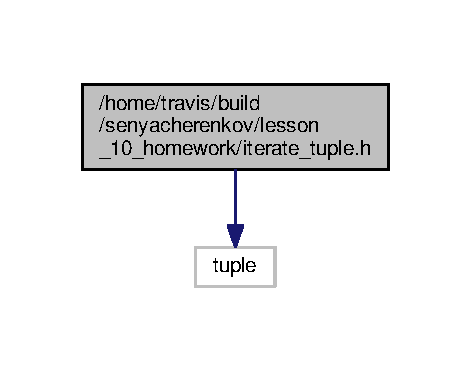
\includegraphics[width=226pt]{iterate__tuple_8h__incl}
\end{center}
\end{figure}
This graph shows which files directly or indirectly include this file\-:
\nopagebreak
\begin{figure}[H]
\begin{center}
\leavevmode
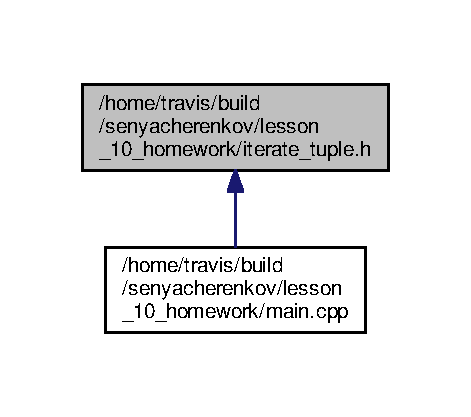
\includegraphics[width=226pt]{iterate__tuple_8h__dep__incl}
\end{center}
\end{figure}
\subsection*{Classes}
\begin{DoxyCompactItemize}
\item 
struct \hyperlink{structhw__utility_1_1iterate__tuple}{hw\-\_\-utility\-::iterate\-\_\-tuple$<$ index, Callback, Args $>$}
\item 
struct \hyperlink{structhw__utility_1_1iterate__tuple_3_010_00_01Callback_00_01Args_8_8_8_4}{hw\-\_\-utility\-::iterate\-\_\-tuple$<$ 0, Callback, Args...$>$}
\item 
struct \hyperlink{structhw__utility_1_1iterate__tuple_3-1_00_01Callback_00_01Args_8_8_8_4}{hw\-\_\-utility\-::iterate\-\_\-tuple$<$-\/1, Callback, Args...$>$}
\end{DoxyCompactItemize}
\subsection*{Namespaces}
\begin{DoxyCompactItemize}
\item 
\hyperlink{namespacehw__utility}{hw\-\_\-utility}
\end{DoxyCompactItemize}
\subsection*{Functions}
\begin{DoxyCompactItemize}
\item 
{\footnotesize template$<$typename Callback , typename... Args$>$ }\\void \hyperlink{iterate__tuple_8h_a743f187bee9ff9e73d38d3a7385625c1}{for\-\_\-each} (std\-::tuple$<$ Args...$>$ \&t, Callback callback)
\end{DoxyCompactItemize}


\subsection{Function Documentation}
\hypertarget{iterate__tuple_8h_a743f187bee9ff9e73d38d3a7385625c1}{\index{iterate\-\_\-tuple.\-h@{iterate\-\_\-tuple.\-h}!for\-\_\-each@{for\-\_\-each}}
\index{for\-\_\-each@{for\-\_\-each}!iterate_tuple.h@{iterate\-\_\-tuple.\-h}}
\subsubsection[{for\-\_\-each}]{\setlength{\rightskip}{0pt plus 5cm}template$<$typename Callback , typename... Args$>$ void for\-\_\-each (
\begin{DoxyParamCaption}
\item[{std\-::tuple$<$ Args...$>$ \&}]{t, }
\item[{Callback}]{callback}
\end{DoxyParamCaption}
)}}\label{iterate__tuple_8h_a743f187bee9ff9e73d38d3a7385625c1}

\hypertarget{main_8cpp}{\section{/home/travis/build/senyacherenkov/lesson\-\_\-10\-\_\-homework/main.cpp File Reference}
\label{main_8cpp}\index{/home/travis/build/senyacherenkov/lesson\-\_\-10\-\_\-homework/main.\-cpp@{/home/travis/build/senyacherenkov/lesson\-\_\-10\-\_\-homework/main.\-cpp}}
}
{\ttfamily \#include $<$iostream$>$}\\*
{\ttfamily \#include $<$string$>$}\\*
{\ttfamily \#include $<$cstdlib$>$}\\*
{\ttfamily \#include $<$vector$>$}\\*
{\ttfamily \#include $<$iterator$>$}\\*
{\ttfamily \#include $<$list$>$}\\*
{\ttfamily \#include $<$utility$>$}\\*
{\ttfamily \#include $<$tuple$>$}\\*
{\ttfamily \#include \char`\"{}iterate\-\_\-tuple.\-h\char`\"{}}\\*
Include dependency graph for main.\-cpp\-:
\nopagebreak
\begin{figure}[H]
\begin{center}
\leavevmode
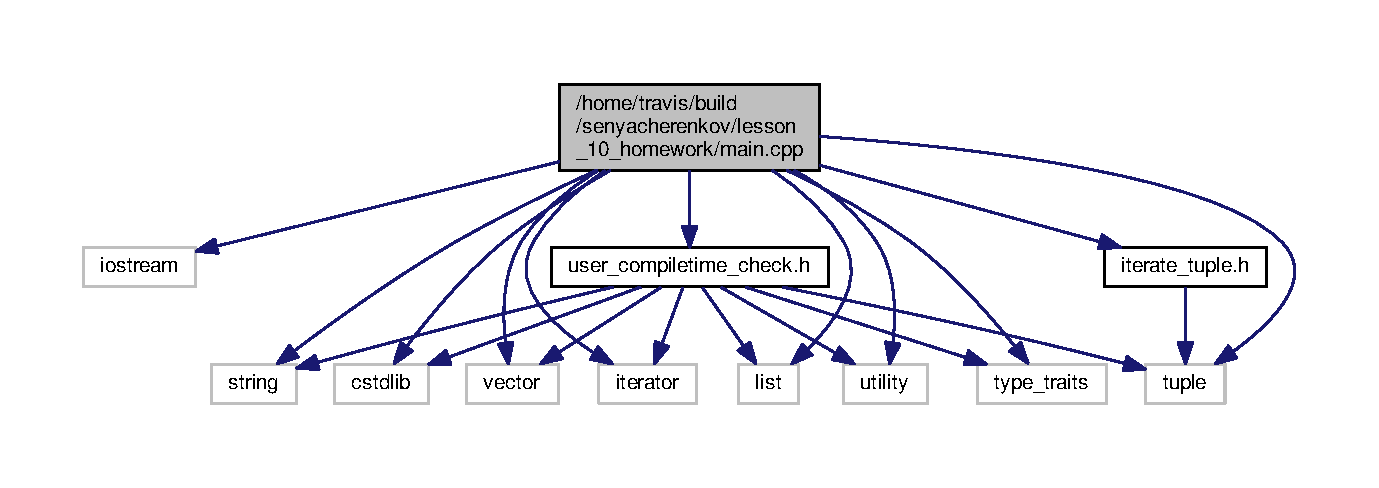
\includegraphics[width=350pt]{main_8cpp__incl}
\end{center}
\end{figure}
\subsection*{Functions}
\begin{DoxyCompactItemize}
\item 
{\footnotesize template$<$typename T\-T $>$ }\\std\-::enable\-\_\-if\\*
$<$ std\-::is\-\_\-integral$<$ typename \\*
std\-::remove\-\_\-reference$<$ T\-T $>$\\*
\-::type $>$\-::value, void $>$\-::type \hyperlink{main_8cpp_ad7b9dbf664b3f8859f6c8b7e0288cddb}{print\-\_\-ip} (T\-T \&input)
\item 
{\footnotesize template$<$$>$ }\\void \hyperlink{main_8cpp_af7b54f6eeea651439ecc070be0e1a690}{print\-\_\-ip$<$ char $>$} (char \&input)
\item 
{\footnotesize template$<$typename T\-T $>$ }\\std\-::enable\-\_\-if\\*
$<$!std\-::is\-\_\-integral$<$ typename \\*
std\-::remove\-\_\-reference$<$ T\-T $>$\\*
\-::type $>$\-::value, void $>$\-::type \hyperlink{main_8cpp_a0a5a690b8b1e96fc11e35796a4ca54fc}{print\-\_\-ip} (T\-T \&input)
\item 
{\footnotesize template$<$typename... Types$>$ }\\void \hyperlink{main_8cpp_aacbe5e8ebd0823963e80b3d31a43d3c4}{print\-\_\-ip} (std\-::tuple$<$ Types...$>$ \&input)
\item 
int \hyperlink{main_8cpp_ae66f6b31b5ad750f1fe042a706a4e3d4}{main} ()
\end{DoxyCompactItemize}


\subsection{Function Documentation}
\hypertarget{main_8cpp_ae66f6b31b5ad750f1fe042a706a4e3d4}{\index{main.\-cpp@{main.\-cpp}!main@{main}}
\index{main@{main}!main.cpp@{main.\-cpp}}
\subsubsection[{main}]{\setlength{\rightskip}{0pt plus 5cm}int main (
\begin{DoxyParamCaption}
{}
\end{DoxyParamCaption}
)}}\label{main_8cpp_ae66f6b31b5ad750f1fe042a706a4e3d4}
\hypertarget{main_8cpp_ad7b9dbf664b3f8859f6c8b7e0288cddb}{\index{main.\-cpp@{main.\-cpp}!print\-\_\-ip@{print\-\_\-ip}}
\index{print\-\_\-ip@{print\-\_\-ip}!main.cpp@{main.\-cpp}}
\subsubsection[{print\-\_\-ip}]{\setlength{\rightskip}{0pt plus 5cm}template$<$typename T\-T $>$ std\-::enable\-\_\-if$<$std\-::is\-\_\-integral$<$typename std\-::remove\-\_\-reference$<$T\-T$>$\-::type$>$\-::value, void$>$\-::type print\-\_\-ip (
\begin{DoxyParamCaption}
\item[{T\-T \&}]{input}
\end{DoxyParamCaption}
)}}\label{main_8cpp_ad7b9dbf664b3f8859f6c8b7e0288cddb}
\hypertarget{main_8cpp_a0a5a690b8b1e96fc11e35796a4ca54fc}{\index{main.\-cpp@{main.\-cpp}!print\-\_\-ip@{print\-\_\-ip}}
\index{print\-\_\-ip@{print\-\_\-ip}!main.cpp@{main.\-cpp}}
\subsubsection[{print\-\_\-ip}]{\setlength{\rightskip}{0pt plus 5cm}template$<$typename T\-T $>$ std\-::enable\-\_\-if$<$!std\-::is\-\_\-integral$<$typename std\-::remove\-\_\-reference$<$T\-T$>$\-::type$>$\-::value, void$>$\-::type print\-\_\-ip (
\begin{DoxyParamCaption}
\item[{T\-T \&}]{input}
\end{DoxyParamCaption}
)}}\label{main_8cpp_a0a5a690b8b1e96fc11e35796a4ca54fc}
\hypertarget{main_8cpp_aacbe5e8ebd0823963e80b3d31a43d3c4}{\index{main.\-cpp@{main.\-cpp}!print\-\_\-ip@{print\-\_\-ip}}
\index{print\-\_\-ip@{print\-\_\-ip}!main.cpp@{main.\-cpp}}
\subsubsection[{print\-\_\-ip}]{\setlength{\rightskip}{0pt plus 5cm}template$<$typename... Types$>$ void print\-\_\-ip (
\begin{DoxyParamCaption}
\item[{std\-::tuple$<$ Types...$>$ \&}]{input}
\end{DoxyParamCaption}
)}}\label{main_8cpp_aacbe5e8ebd0823963e80b3d31a43d3c4}
\hypertarget{main_8cpp_af7b54f6eeea651439ecc070be0e1a690}{\index{main.\-cpp@{main.\-cpp}!print\-\_\-ip$<$ char $>$@{print\-\_\-ip$<$ char $>$}}
\index{print\-\_\-ip$<$ char $>$@{print\-\_\-ip$<$ char $>$}!main.cpp@{main.\-cpp}}
\subsubsection[{print\-\_\-ip$<$ char $>$}]{\setlength{\rightskip}{0pt plus 5cm}template$<$$>$ void {\bf print\-\_\-ip}$<$ char $>$ (
\begin{DoxyParamCaption}
\item[{char \&}]{input}
\end{DoxyParamCaption}
)}}\label{main_8cpp_af7b54f6eeea651439ecc070be0e1a690}

\hypertarget{README_8md}{\section{/home/travis/build/senyacherenkov/lesson\-\_\-10\-\_\-homework/\-R\-E\-A\-D\-M\-E.md File Reference}
\label{README_8md}\index{/home/travis/build/senyacherenkov/lesson\-\_\-10\-\_\-homework/\-R\-E\-A\-D\-M\-E.\-md@{/home/travis/build/senyacherenkov/lesson\-\_\-10\-\_\-homework/\-R\-E\-A\-D\-M\-E.\-md}}
}

%--- End generated contents ---

% Index
\newpage
\phantomsection
\addcontentsline{toc}{chapter}{Index}
\printindex

\end{document}
